% Options for packages loaded elsewhere
\PassOptionsToPackage{unicode}{hyperref}
\PassOptionsToPackage{hyphens}{url}
%
\documentclass[
  8pt,
  ignorenonframetext,
]{beamer}
\usepackage{pgfpages}
\setbeamertemplate{caption}[numbered]
\setbeamertemplate{caption label separator}{: }
\setbeamercolor{caption name}{fg=normal text.fg}
\beamertemplatenavigationsymbolsempty
% Prevent slide breaks in the middle of a paragraph
\widowpenalties 1 10000
\raggedbottom
\setbeamertemplate{part page}{
  \centering
  \begin{beamercolorbox}[sep=16pt,center]{part title}
    \usebeamerfont{part title}\insertpart\par
  \end{beamercolorbox}
}
\setbeamertemplate{section page}{
  \centering
  \begin{beamercolorbox}[sep=12pt,center]{part title}
    \usebeamerfont{section title}\insertsection\par
  \end{beamercolorbox}
}
\setbeamertemplate{subsection page}{
  \centering
  \begin{beamercolorbox}[sep=8pt,center]{part title}
    \usebeamerfont{subsection title}\insertsubsection\par
  \end{beamercolorbox}
}
\AtBeginPart{
  \frame{\partpage}
}
\AtBeginSection{
  \ifbibliography
  \else
    \frame{\sectionpage}
  \fi
}
\AtBeginSubsection{
  \frame{\subsectionpage}
}
\usepackage{amsmath,amssymb}
\usepackage{lmodern}
\usepackage{iftex}
\ifPDFTeX
  \usepackage[T1]{fontenc}
  \usepackage[utf8]{inputenc}
  \usepackage{textcomp} % provide euro and other symbols
\else % if luatex or xetex
  \usepackage{unicode-math}
  \defaultfontfeatures{Scale=MatchLowercase}
  \defaultfontfeatures[\rmfamily]{Ligatures=TeX,Scale=1}
\fi
% Use upquote if available, for straight quotes in verbatim environments
\IfFileExists{upquote.sty}{\usepackage{upquote}}{}
\IfFileExists{microtype.sty}{% use microtype if available
  \usepackage[]{microtype}
  \UseMicrotypeSet[protrusion]{basicmath} % disable protrusion for tt fonts
}{}
\makeatletter
\@ifundefined{KOMAClassName}{% if non-KOMA class
  \IfFileExists{parskip.sty}{%
    \usepackage{parskip}
  }{% else
    \setlength{\parindent}{0pt}
    \setlength{\parskip}{6pt plus 2pt minus 1pt}}
}{% if KOMA class
  \KOMAoptions{parskip=half}}
\makeatother
\usepackage{xcolor}
\newif\ifbibliography
\usepackage{longtable,booktabs,array}
\usepackage{calc} % for calculating minipage widths
\usepackage{caption}
% Make caption package work with longtable
\makeatletter
\def\fnum@table{\tablename~\thetable}
\makeatother
\setlength{\emergencystretch}{3em} % prevent overfull lines
\providecommand{\tightlist}{%
  \setlength{\itemsep}{0pt}\setlength{\parskip}{0pt}}
\setcounter{secnumdepth}{-\maxdimen} % remove section numbering
\newlength{\cslhangindent}
\setlength{\cslhangindent}{1.5em}
\newlength{\csllabelwidth}
\setlength{\csllabelwidth}{3em}
\newlength{\cslentryspacingunit} % times entry-spacing
\setlength{\cslentryspacingunit}{\parskip}
\newenvironment{CSLReferences}[2] % #1 hanging-ident, #2 entry spacing
 {% don't indent paragraphs
  \setlength{\parindent}{0pt}
  % turn on hanging indent if param 1 is 1
  \ifodd #1
  \let\oldpar\par
  \def\par{\hangindent=\cslhangindent\oldpar}
  \fi
  % set entry spacing
  \setlength{\parskip}{#2\cslentryspacingunit}
 }%
 {}
\usepackage{calc}
\newcommand{\CSLBlock}[1]{#1\hfill\break}
\newcommand{\CSLLeftMargin}[1]{\parbox[t]{\csllabelwidth}{#1}}
\newcommand{\CSLRightInline}[1]{\parbox[t]{\linewidth - \csllabelwidth}{#1}\break}
\newcommand{\CSLIndent}[1]{\hspace{\cslhangindent}#1}
% type setting
% ------------------------------------------------------------------------------
\usepackage[german]{babel}     

% fonts
% ------------------------------------------------------------------------------
\usefonttheme{professionalfonts}

% slide title and horizontal line
% ------------------------------------------------------------------------------
\setbeamertemplate{frametitle}{%
    \vskip-30pt \color{black}\large%
    \begin{minipage}[b][23pt]{120mm}%
    \flushleft\insertframetitle%
    \end{minipage}%
}

\setbeamertemplate{headline}										
{
\vskip10pt\hfill\hspace{3.5mm} 										 
\vskip15pt\color{black}\rule{\textwidth}{0.4pt} 					 
}

% slide number
% ---------------------------------------------------------------
\setbeamertemplate{navigation symbols}{}
\setbeamertemplate{footline}
{
\vskip5pt
\vskip2pt
\makebox[123mm]{\hspace{7.5mm}
\hfill Wahrscheinlichkeitstheorie und Frequentistische Inferenz $\vert$ 
\copyright $ $ 2023 Dirk Ostwald CC BY-NC-SA 4.0 $\vert$ 
Folie \insertframenumber}
\vskip4pt
}

% block color scheme
% ------------------------------------------------------------------------------
% colors
\definecolor{white}{RGB}{255,255,255}
\definecolor{grey}{RGB}{235,235,235}
\definecolor{lightgrey}{RGB}{245,245,245}
\definecolor{LightBlue}{RGB}{220,220,255}
\definecolor{darkblue}{RGB}{51, 51, 153}

% definitions and theorems
\setbeamercolor{block title}{fg = black, bg = grey}
\setbeamercolor{block body}{fg = black, bg = lightgrey}

% general line spacing 
% ------------------------------------------------------------------------------
\linespread{1.3}

% local line spacing
% ------------------------------------------------------------------------------
\usepackage{setspace}

% colors
% -----------------------------------------------------------------------------
\usepackage{color}

% justified text
% ------------------------------------------------------------------------------
\usepackage{ragged2e}
\usepackage{etoolbox}
\apptocmd{\frame}{}{\justifying}{}
\usepackage{ragged2e}
\renewcommand{\raggedright}{\justifying}

% bullet point lists
% -----------------------------------------------------------------------------
\setbeamertemplate{itemize item}[circle]
\setbeamertemplate{itemize subitem}[circle]
\setbeamertemplate{itemize subsubitem}[circle]
\setbeamercolor{itemize item}{fg = black}
\setbeamercolor{itemize subitem}{fg = black}
\setbeamercolor{itemize subsubitem}{fg = black}
\setbeamercolor{enumerate item}{fg = black}
\setbeamercolor{enumerate subitem}{fg = black}
\setbeamercolor{enumerate subsubitem}{fg = black}
\setbeamerfont{itemize/enumerate body}{}
\setbeamerfont{itemize/enumerate subbody}{size = \normalsize}
\setbeamerfont{itemize/enumerate subsubbody}{size = \normalsize}

% color links
% ------------------------------------------------------------------------------
\usepackage{hyperref}
\definecolor{urls}{RGB}{204,0,0}
\hypersetup{colorlinks, citecolor = darkblue, urlcolor = urls}


% additional math commands
% ------------------------------------------------------------------------------
\usepackage{bm}                                         % bold math symbols
\newcommand{\niton}{\not\owns}

% text highlighting
% ------------------------------------------------------------------------------
\usepackage{soul}
\makeatletter
\let\HL\hl
\renewcommand\hl{%
  \let\set@color\beamerorig@set@color
  \let\reset@color\beamerorig@reset@color
  \HL}
\makeatother

% equation highlighting
% -----------------------------------------------------------------------------
\newcommand{\highlight}[2][yellow]{\mathchoice%
  {\colorbox{#1}{$\displaystyle#2$}}%
  {\colorbox{#1}{$\textstyle#2$}}%
  {\colorbox{#1}{$\scriptstyle#2$}}%
  {\colorbox{#1}{$\scriptscriptstyle#2$}}}%

% additional mathematical operators
% ------------------------------------------------------------------------------
\DeclareMathOperator*{\argmax}{arg\,max}
\DeclareMathOperator*{\argmin}{arg\,min}

\ifLuaTeX
  \usepackage{selnolig}  % disable illegal ligatures
\fi
\IfFileExists{bookmark.sty}{\usepackage{bookmark}}{\usepackage{hyperref}}
\IfFileExists{xurl.sty}{\usepackage{xurl}}{} % add URL line breaks if available
\urlstyle{same} % disable monospaced font for URLs
\hypersetup{
  hidelinks,
  pdfcreator={LaTeX via pandoc}}

\author{}
\date{\vspace{-2.5em}}

\begin{document}

\begin{frame}[plain]{}
\protect\hypertarget{section}{}
\center

\begin{center}
\includegraphics[width=0.2\linewidth]{2_Abbildungen/wtfi_2_otto} \end{center}

\vspace{2mm}

\Large

Wahrscheinlichkeitstheorie und Frequentistische Inferenz \vspace{6mm}

\large

BSc Psychologie WiSe 2021/22

\vspace{6mm}
\large

Prof.~Dr.~Dirk Ostwald
\end{frame}

\begin{frame}[plain]{}
\protect\hypertarget{section-1}{}
\vfill
\center
\huge

\textcolor{black}{(2) Wahrscheinlichkeitsräume} \vfill
\end{frame}

\begin{frame}{}
\protect\hypertarget{section-2}{}
\center
\huge

\textcolor{darkblue}{Statistik} \vspace{5mm}

\Large

Die Kunst, aus Daten Sinn zu generieren

\textbf{und seine assoziierte Unsicherheit zu quantifizieren}
\end{frame}

\begin{frame}{}
\protect\hypertarget{section-3}{}
\begin{center}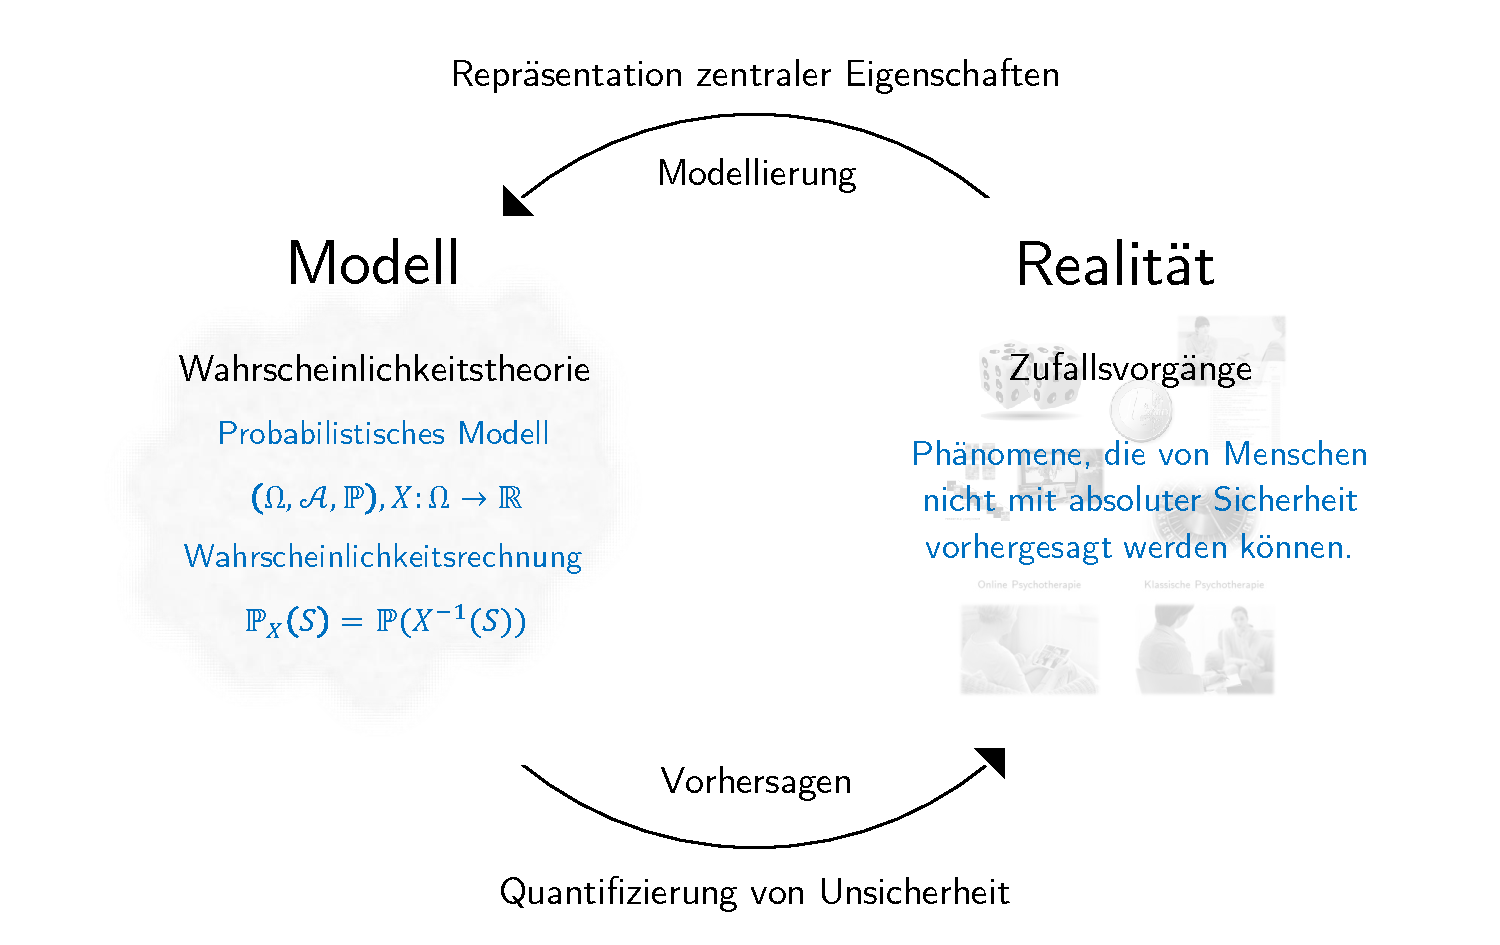
\includegraphics[width=1\linewidth]{2_Abbildungen/wtfi_2_wahrscheinlichkeitstheorie_modell} \end{center}
\end{frame}

\begin{frame}{}
\protect\hypertarget{section-4}{}
\begin{center}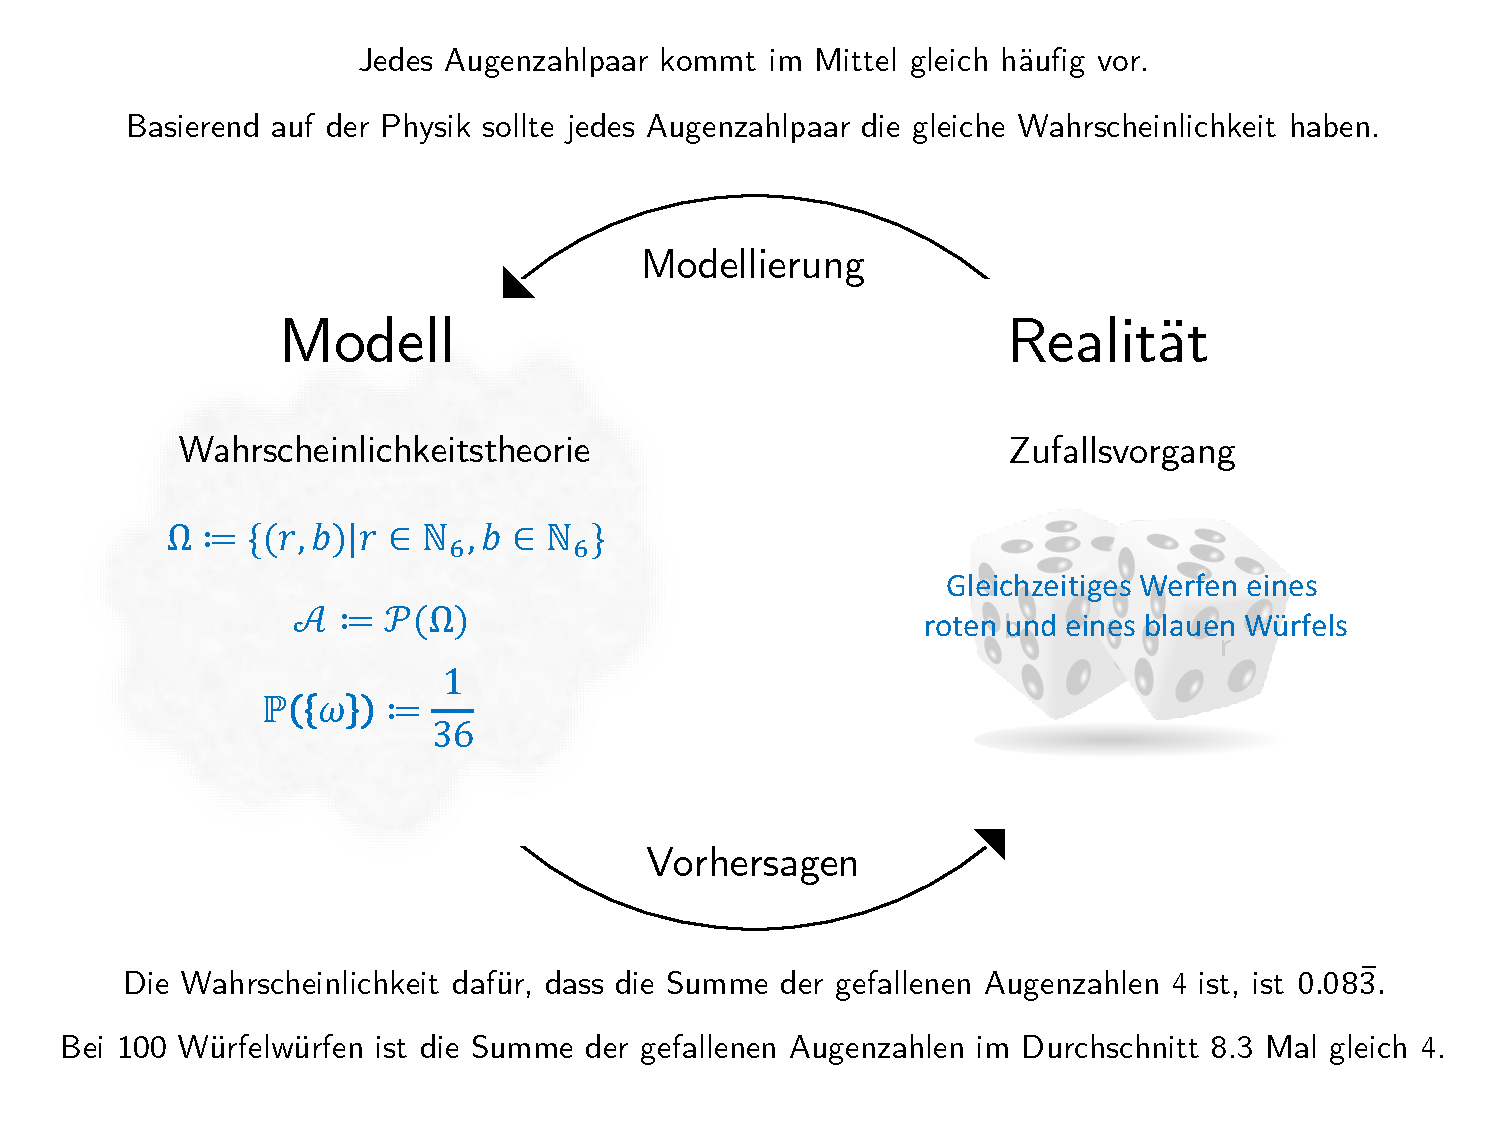
\includegraphics[width=1\linewidth]{2_Abbildungen/wtfi_2_wahrscheinlichkeitstheorie_modell_beispiel} \end{center}
\end{frame}

\begin{frame}{}
\protect\hypertarget{section-5}{}
\setstretch{2.5}
\large
\vfill

Definition

Erste Eigenschaften

Wahrscheinlichkeitsfunktionen

Beispiele

Selbstkontrollfragen \vfill
\end{frame}

\begin{frame}{}
\protect\hypertarget{section-6}{}
\setstretch{2.5}
\large
\vfill

\textbf{Definition}

Erste Eigenschaften

Wahrscheinlichkeitsfunktionen

Beispiele

Selbstkontrollfragen \vfill
\end{frame}

\begin{frame}{Definition}
\protect\hypertarget{definition}{}
\small
\begin{definition}[Wahrscheinlichkeitsraum]
\justifying
Ein \textit{Wahrscheinlichkeitsraum} ist ein Triple $(\Omega, \mathcal{A}, \mathbb{P})$, wobei
\begin{itemize}
\item $\Omega$ eine beliebige nichtleere Menge von \textit{Ergebnissen} $\omega$ ist und \textit{Ergebnismenge} heißt,
\item $\mathcal{A}$ eine \textit{$\sigma$-Algebra auf $\Omega$} ist und \textit{Ereignissystem} heißt,
\item $\mathbb{P}$ eine Abbildung der Form $\mathbb{P}:\mathcal{A} \to [0,1]$ mit den Eigenschaften 
\begin{itemize}
\begin{small}
\item[o] \textit{Nicht-Negativität} $\mathbb{P}(A) \ge 0$ für alle $A \in \mathcal{A}$,
\item[o] \textit{Normiertheit} $\mathbb{P}(\Omega) = 1$ und
\item[o] \textit{ $\sigma$-Additivität} $\mathbb{P}(\cup_{i=1}^\infty A_i) = \sum\limits_{i=1}^\infty \mathbb{P}(A_i)$
          für paarweise disjunkte $A_i \in \mathcal{A}$
\end{small}
\end{itemize}
ist und \textit{Wahrscheinlichkeitsmaß} heißt. 
\end{itemize}
Das Tuple $(\Omega, \mathcal{A})$ aus Ergebnismenge und Ereignissystem wird 
als \textit{Messraum} bezeichnet.
\end{definition}

Bemerkung

\begin{itemize}
\tightlist
\item
  Die Definition benutzt den Begriff der \textit{$\sigma$-Algebra}.
\end{itemize}
\end{frame}

\begin{frame}{Definition}
\protect\hypertarget{definition-1}{}
\small
\begin{definition}[$\sigma$-Algebra]
\justifying
$\Omega$ sei eine Menge und $\mathcal{A}$ sei eine Menge von Teilmengen von $\Omega$.
$\mathcal{A}$ heißt \textit{$\sigma$-Algebra auf $\Omega$}, wenn
\begin{itemize}
\begin{small}
\item $\Omega \in \mathcal{A}$ ist,
\item $\mathcal{A}$ abgeschlossen unter der Bildung von Komplementärmengen ist, 
    also wenn für alle $A\in \mathcal{A}$ gilt, dass auch $A^c := \Omega \setminus A \in \mathcal{A}$ ist, 
\item $\mathcal{A}$ abgeschlossen unter der abzählbaren Vereinigung von Ereignissen ist, also wenn aus  
    $A_1,A_2,... \in \mathcal{A}$ folgt, dass auch $\cup_{i=1}^\infty A_i \in \mathcal{A}$ ist.  
\end{small}
\end{itemize}
\end{definition}

Bemerkungen

\begin{itemize}
\tightlist
\item
  Eine \(\sigma\)-Algebra ist eine Menge von Mengen.
\item
  Eine als bekannt vorausgesetzte andere Menge von Mengen ist die
  \emph{Potenzmenge}.
\item
  Mengen von Mengen heißen auch \emph{Mengensysteme}.
\end{itemize}
\end{frame}

\begin{frame}{Definition}
\protect\hypertarget{definition-2}{}
\begin{minipage}{.29\linewidth}
\begin{center}
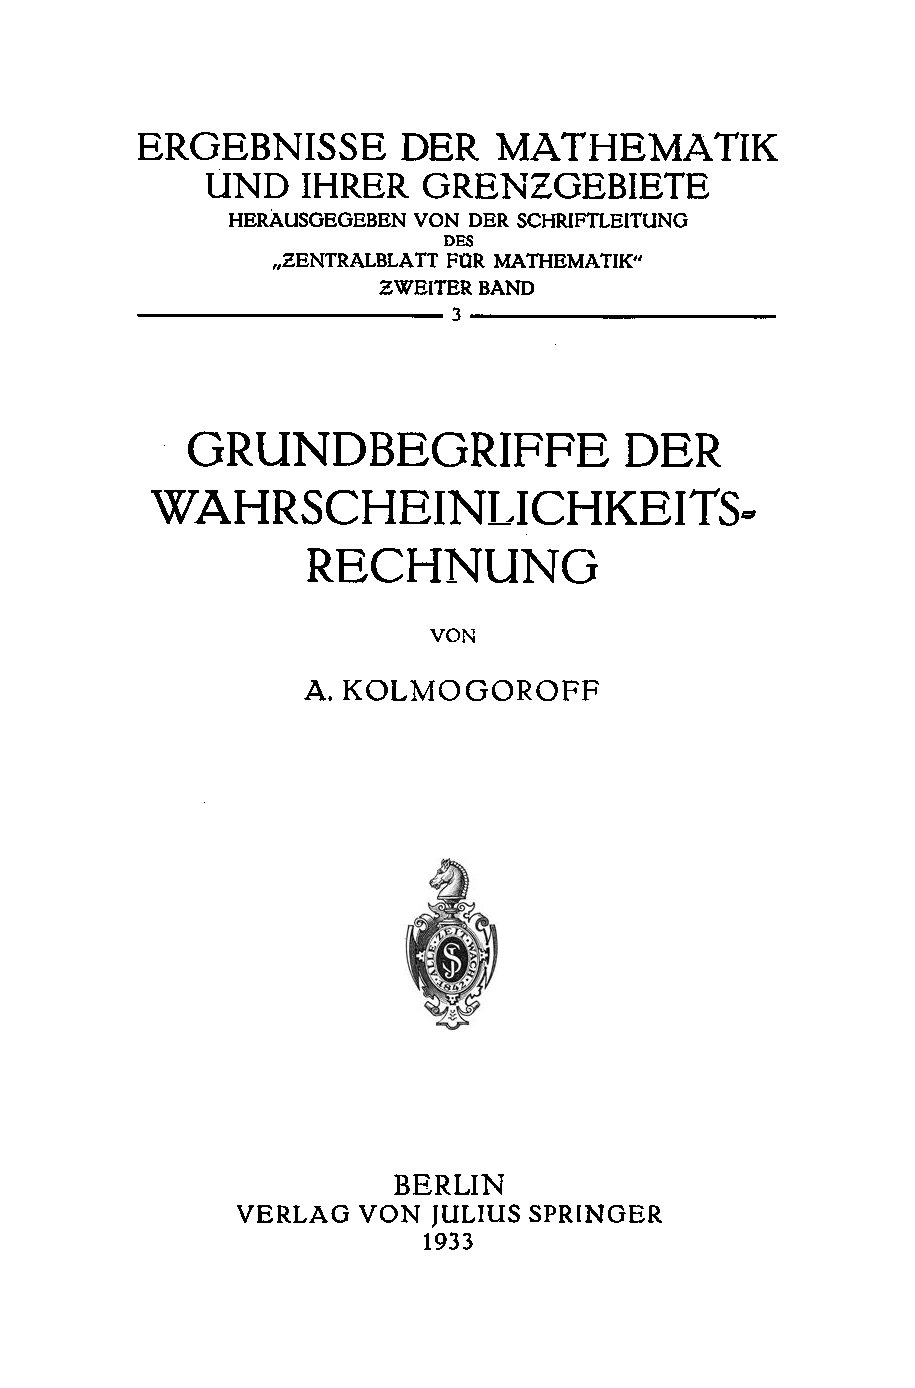
\includegraphics[scale=.25]{2_Abbildungen/wtfi_2_kolmogorov_1.pdf}
\end{center}
\end{minipage}
\begin{minipage}{.29\linewidth}
\begin{center}
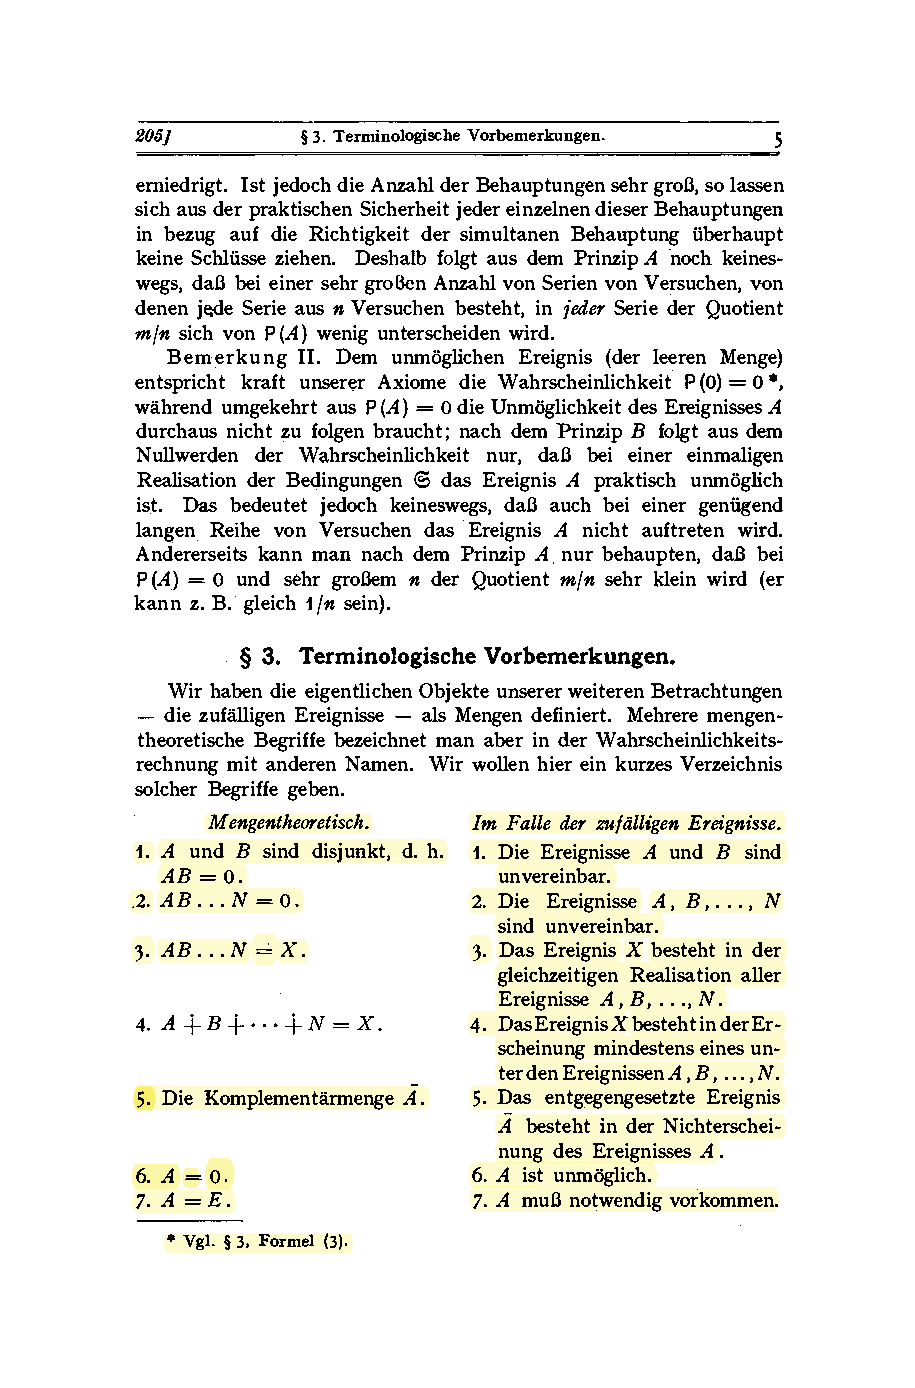
\includegraphics[scale=.25]{2_Abbildungen/wtfi_2_kolmogorov_2.pdf}
\end{center}
\end{minipage}
\begin{minipage}{.29\linewidth}
\begin{center}
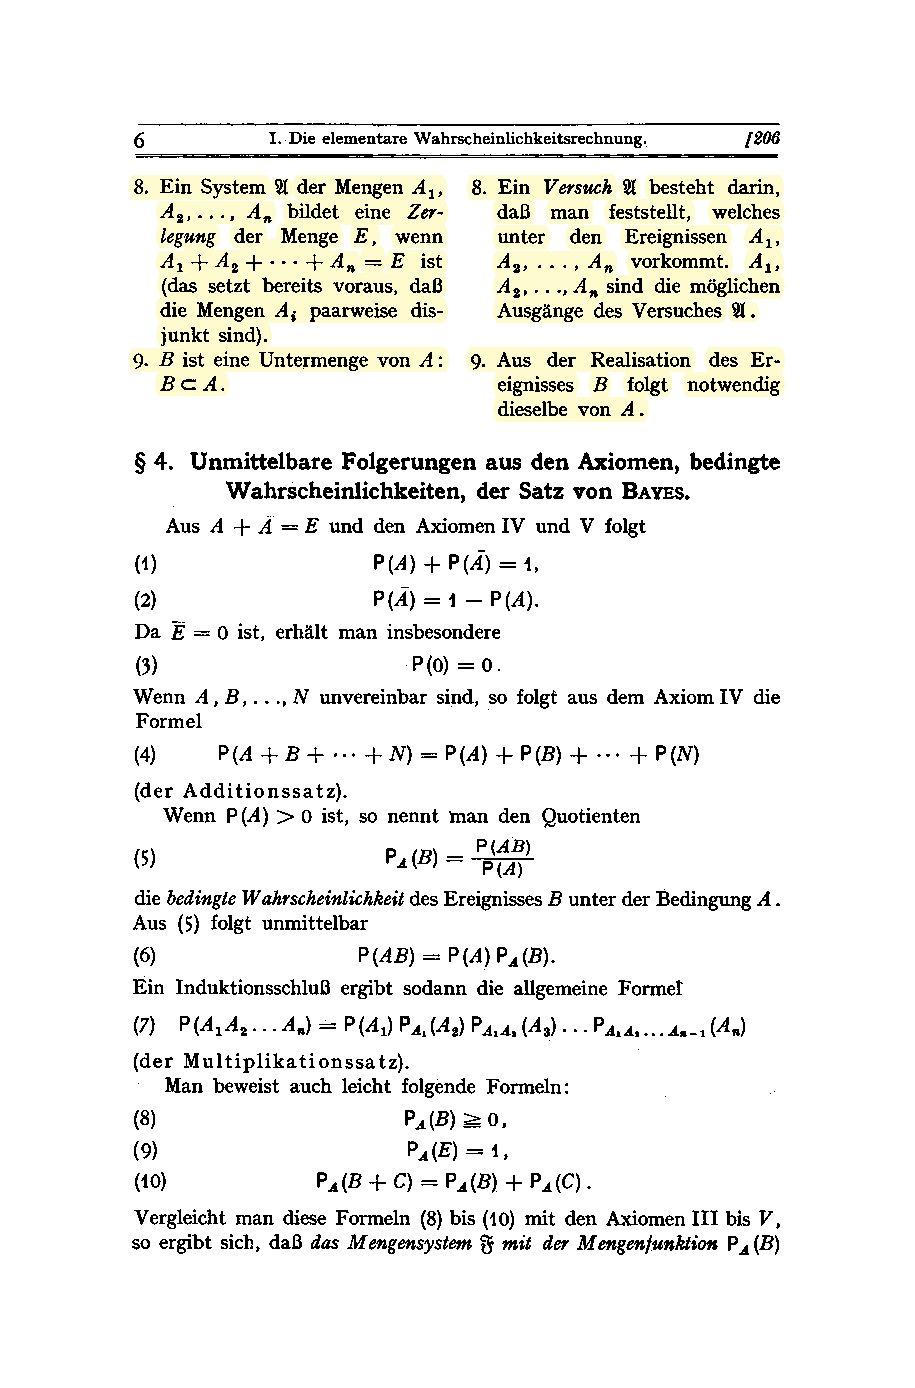
\includegraphics[scale=.25]{2_Abbildungen/wtfi_2_kolmogorov_3.pdf}
\end{center}
\end{minipage}

\footnotesize
\setstretch{1}

``Zweck des vorliegenden Heftes ist eine axiomatische Begründung der
Wahrscheinlichkeitsrechnung. Der leitende Gedanke des Verfassers war
dabei, die Grundbegriffe der Wahrscheinlichkeitsrechnung, welche noch
unlängst für ganz eigenartig galten, natürlicherweise in die Reihe der
allgemeinen Begriffsbildungen der modernen Mathematik {[}Mengen,
Abbildungen{]} einzuordnen.''

``Wir haben die eigentlichen Objekte unserer weiteren Betrachtungen -
die zufälligen Ereignisse - als Mengen definiert.''

\flushright

Kolmogoroff (1933) {[}*1903 \textdagger 1987{]}
\end{frame}

\begin{frame}{Definition}
\protect\hypertarget{definition-3}{}
\setstretch{1.6}

\textcolor{darkblue}{Ergebnismenge $\Omega$} \small

\begin{itemize}
\tightlist
\item
  Wir betrachten zunächst \emph{endliche Wahrscheinlichkeitsräume} mit
  \(|\Omega|<\infty\).
\item
  \(\Omega\) habe also nur endlich viele (``diskrete'') Elemente.
\item
  Zum Modellieren des Werfen eines Würfels definiert man z.B.
  \(\Omega := \{1,2,3,4,5,6\}\).
\end{itemize}

\vspace{5mm}
\normalsize

\textcolor{darkblue}{Die stillschweigende Mechanik des Wahrscheinlichkeitsraummodells}
\small

\begin{itemize}
\tightlist
\item
  Wir stellen uns sequentielle \emph{Durchgänge} eines
  \emph{Zufallsvorgangs} vor.
\item
  In jedem Durchgang wird genau ein \(\omega\) aus \(\Omega\) mit
  Wahrscheinlichkeit \(\mathbb{P}(\{\omega\})\) \emph{realisiert}.
\item
  \(\mathbb{P}(\{\omega\})\) bestimmt, mit welcher Wahrscheinlichkeit
  \(\omega\) in einem Durchgang aus \(\Omega\) realisiert wird.
\item
  Beim Modell des Werfens eines fairen Würfels gilt etwa
  \(\mathbb{P}(\{\omega\}) = 1/6\) für alle \(\omega \in \Omega\).
\item
  Im 1. Durchgang wird z.B. ``\(4\)'' realisiert, im 2. Durchgang
  ``\(1\)'', im 3. Durchgang ``\(5\)'', usw.
\end{itemize}
\end{frame}

\begin{frame}{Definition}
\protect\hypertarget{definition-4}{}
\textcolor{darkblue}{Ereignisse $A \in \mathcal{A}$} \small
\setstretch{1.7}

\begin{itemize}
\tightlist
\item
  \emph{Ereignisse} stellt man sich am besten als Zusammenfassung (ein
  oder) mehrerer Ergebnisse vor.
\item
  Beim Werfen eines Würfels sind mögliche Ereignisse zum Beispiel
\end{itemize}

\begin{center}
\begin{tabular}{ll}
Es fällt eine gerade Augenzahl,          & das heißt $\omega \in \{2,4,6\}$      \\
Es fällt eine Augenzahl größer als Zwei, & das heißt $\omega \in \{3,4,5,6\}$   \\
Es fällt eine Eins oder eine Fünf,       & das heißt $\omega \in \{1,5\}$
\end{tabular}
\end{center}

\begin{itemize}
\tightlist
\item
  Natürlich sind auch die Ergebnisse \(\omega \in \Omega\) mögliche
  Ereignisse zum Beispiel
\end{itemize}

\begin{center}
\begin{tabular}{ll}
Es fällt eine Eins,                      & das heißt $\omega \in \{1\}$          \\
Es fällt eine Sechs,                     & das heißt $\omega \in \{6\}$          \\
\end{tabular}
\end{center}

\begin{itemize}
\tightlist
\item
  Betrachtet man \(\omega \in \Omega\) als Ereignis, so nennt man es
  \emph{Elementarereignis} und schreibt \(\{\omega\}\).
\end{itemize}

\footnotesize

``Wir haben die eigentlichen Objekte unserer weiteren Betrachtungen -
die zufälligen Ereignisse - als Mengen definiert.''

\flushright

Kolmogoroff (1933) {[}*1903 \textdagger 1987{]}
\end{frame}

\begin{frame}{Definition}
\protect\hypertarget{definition-5}{}
\textcolor{darkblue}{Ereignissystem $\mathcal{A}$} \small
\setstretch{1.1}

\begin{itemize}
\justifying
\itemsep1mm
\item Sinn des Ereignissystems ist es, alle Ereignisse, die sich basierend auf einer 
gegebenen Ergebnismenge bei Auswahl eines $\omega \in \Omega$ ergeben können, 
mathematisch zu repräsentieren.
\item Das Ereignissystem $\mathcal{A}$ ist die vollständige Menge aller möglichen Ereignisse bei gegebenem $\Omega$.
\item Die Forderung, dass $\mathcal{A}$ die $\sigma$-Algebra Kriterien erfüllt, begründet sich wie folgt
\begin{itemize}

\begin{footnotesize}
\setstretch{1.1}
\item[$\circ$] \justifying Es soll sichergestellt sein, dass $\omega \in \Omega$ für
beliebiges $\omega$, dass also irgendein Ergebnis realisiert wird, eines der möglichen Ereignisse ist.
Dies entspricht $\Omega \in \mathcal{A}$. Zu jedem Ereignis soll es auch möglich sein, 
dass dieses Ereignis gerade nicht eintritt. Dies entspricht, dass aus $A \in \mathcal{A}$ 
folgen soll, dass $A^c = \Omega \setminus A$ auch in $\mathcal{A}$ ist. Dies 
impliziert auch, dass $\emptyset = \Omega \setminus \Omega \in \mathcal{A}$. 
Ein Ereignis ist also, dass kein Elementarereignis eintritt, allerdings passiert 
dies nur mit Wahrscheinlichkeit Null, $\mathbb{P}(\emptyset) = 0$. Es tritt also 
sicher immer ein Elementarereignis ein. Die Kombination von Ereignissen soll auch 
immer ein Ereignis sein, z.B. ``Es fällt eine gerade Zahl'' und/oder ``Es fällt
eine Zahl größer 2''. Dies entspricht, dass aus $A_1,A_2,... \in \mathcal{A} $ 
folgen soll, dass auch $\cup_{i=1}^\infty A_i \in \mathcal{A}$.
\end{footnotesize}

\end{itemize}
\item Für endliches $\Omega$ und für $\Omega := \mathbb{R}$ sind passende Ereignissysteme schon lange bekannt.
\center
\begin{tabular}{rl}
$\Omega$ ist endlich        & $\Rightarrow$ Man wählt für $\mathcal{A}$ die Potenzmenge von $\Omega$ \\
$\Omega$ ist $\mathbb{R}$   & $\Rightarrow$ Man wählt für $\mathcal{A}$ die \textit{Borelsche $\sigma$-Algebra $\mathcal{B}(\mathbb{R})$} \\
$\Omega$ ist $\mathbb{R}^n$ & $\Rightarrow$ Man wählt für $\mathcal{A}$ die \textit{Borelsche $\sigma$-Algebra $\mathcal{B}(\mathbb{R}^n)$}
\end{tabular}
\end{itemize}
\end{frame}

\begin{frame}{Definition}
\protect\hypertarget{definition-6}{}
\small
\begin{theorem}[Ereignissystem bei endlicher Ergebnismenge]
\justifying
\normalfont
$\Omega := \{\omega_1,\omega_2,...,\omega_n\}$ mit $n \in \mathbb{N}$  sei eine endliche
Menge. Dann ist die Potenzmenge $\mathcal{P}(\Omega)$ von $\Omega$ eine 
$\sigma$-Algebra auf $\Omega$ und damit ein geeignetes Ereignisssytem im 
Wahrscheinlichkeitsraummodell.
\end{theorem}

\footnotesize

\underline{Beweis} \justifying

Die Potenzmenge von \(\Omega\) ist die Menge aller Teilmengen von
\(\Omega\). Wir überprüfen die \(\sigma\)-Algebra Eigenschaften.
Zunächst gilt, dass \(\Omega\) selbst eine der Teilmengen von \(\Omega\)
ist, also ist die erste \(\sigma\)-Algebra Eigenschaft erfüllt. Sei nun
\(A\) eine Teilmenge von \(\Omega\). Dann ist auch
\(A^c = \Omega \setminus A\) eine Teilmenge von \(\Omega\) und somit ist
auch die zweite \(\sigma\)-Algebra Eigenschaft erfüllt. Schließlich
betrachten wir die Vereinigung von \(n\) Teilmengen
\(A_1, A_2, ...,A_n \subseteq \Omega\). Dann ist \(\cup_{i=1}^n A_i\)
die Menge der \(\omega \in \Omega\) für die gilt, dass
\(\omega \in A_1\) und/oder \(\omega \in A_2\) \ldots{} und/oder
\(\omega \in A_n\). Da für alle diese \(\omega\) gilt, dass
\(\omega \in \Omega\) ist also auch \(\cup_{i=1}^n A_i\) eine Teilmenge
von \(\Omega\) und damit auch die dritte \(\sigma\)-Algebra Eigenschaft
erfüllt.

\vfill
\end{frame}

\begin{frame}{Definition}
\protect\hypertarget{definition-7}{}
\setstretch{2}

\textcolor{darkblue}{Wahrscheinlichkeitsmaß $\mathbb{P}$}

\small

\begin{itemize}
\tightlist
\item
  \justifying \((\Omega,\mathcal{A})\) ist die \emph{strukturelle Basis}
  eines Wahrscheinlichkeitsraummmodells.
\item
  \(\mathbb{P}\) repräsentiert die probabilistischen Charakteristika
  eines Wahrscheinlichkeitsraummodells.
\item
  \(\mathbb{P}\) entspricht also der \emph{funktionellen Basis} eines
  Wahrscheinlichkeitsraummmodells.
\item
  Es gilt \(\mathbb{P}: \mathcal{A} \to [0,1]\), \(\mathbb{P}\) ordnet
  also (nur) Mengen Wahrscheinlichkeiten zu.
\item
  Mit \(\{\omega\} \in \mathcal{A}\, \forall\, \omega \in \Omega\)
  ordnet \(\mathbb{P}\) auch den Elementareignissen Wahrscheinlichkeiten
  zu.
\item
  Wahrscheinlichkeiten sind Zahlen in \([0,1]\), nicht Prozente (20\%)
  oder Verhältnisse (50:50).
\item
  \(\mathbb{P}(\Omega) = 1\) entspricht der Tatsache, dass in jedem
  Durchgang sicher \(\omega \in \Omega\) gilt.
\item
  In jedem Durchgang eines Zufallsvorgangs tritt also zumindest ein
  Elementarereignis ein.
\end{itemize}
\end{frame}

\begin{frame}{Definition}
\protect\hypertarget{definition-8}{}
\textcolor{darkblue}{$\sigma$-Additivität des Wahrscheinlichkeitsmaßes $\mathbb{P}$}
\small

\begin{itemize}
\justifying
\itemsep2mm
\item Die $\sigma$-Additivität von $\mathbb{P}$ erlaubt es, aus bereits bekannten
  Ereigniswahrscheinlichkeiten die Wahrscheinlichkeiten anderer Ereignisse zu berechnen.
\item Die $\sigma$-Additivität ist also die Grundlage für das Rechnen mit Wahrscheinlichkeiten,
  das heißt für die \textit{Wahrscheinlichkeitsrechnung}.
\item Man kann basierend auf einer Definition von $\Omega, \mathcal{A}$ und $\mathbb{P}$ also
  Wahrscheinlichkeiten für alle möglichen Ereignisse eines Wahrscheinlichkeitsraummodells berechnen.
  Ob diese Wahrscheinlichkeiten aber tatsächlich etwas mit den realen Ereignissen 
  in einem Zufallsvorgang zu tun haben, kommt darauf an, ob die Modellierung 
  einigermaßen gelungen ist oder nicht.
\item Die hergeleiteten Wahrscheinlichkeiten werden zumindest nach den Regeln der Vernunft, 
  also der Logik und der Mathematik, d.h. rational bestimmt.
\item Insgesamt erlaubt das Wahrscheinlichkeitsmodell also das modellbasierte 
  schlussfolgernde Denken über mit Unsicherheit behaftete Phänomene
\end{itemize}

\center
\normalsize

\textcolor{darkblue}{Probability Theory $\Leftrightarrow$ Reasoning with Uncertainty}
\end{frame}

\begin{frame}{}
\protect\hypertarget{section-7}{}
\setstretch{2.5}
\large
\vfill

Definition

\textbf{Erste Eigenschaften}

Wahrscheinlichkeitsfunktionen

Beispiele

Selbstkontrollfragen \vfill
\end{frame}

\begin{frame}{Erste Eigenschaften}
\protect\hypertarget{erste-eigenschaften}{}
\setstretch{1.2}
\small
\begin{theorem}[Wahrscheinlichkeit des unmöglichen Ereignisses]
\justifying
\normalfont
$(\Omega, \mathcal{A}, \mathbb{P})$ sei ein Wahrscheinlichkeitsraum. Dann gilt
\begin{equation}
\mathbb{P}(\emptyset) = 0.
\end{equation}
\end{theorem}

\footnotesize

\underline{Beweis}

Für \(i = 1,2,...\) sei \(A_i := \emptyset\). Dann ist \(A_1,A_2,...\)
eine Folge disjunkter Ereignisse, weil gilt, dass
\(\emptyset \cap \emptyset = \emptyset\) und es ist
\(\cup_{i=1}^\infty A_i = \emptyset\). Mit der \(\sigma\)-Additivität
von \(\mathbb{P}\) folgt dann, dass \begin{equation}
\mathbb{P}(\emptyset)
= \mathbb{P}\left(\cup_{i=1}^\infty A_i\right)
= \sum_{i=1}^\infty \mathbb{P}\left(A_i\right)
= \sum_{i=1}^\infty \mathbb{P}\left(\emptyset\right)
\end{equation} Das unendliche Aufaddieren der Zahl
\(\mathbb{P}(\emptyset) \in [0,1]\) soll also wieder
\(\mathbb{P}(\emptyset)\) ergeben. Dies ist aber nur möglich, wenn
\(\mathbb{P}(\emptyset) = 0\).

\(\hfill\Box\)
\end{frame}

\begin{frame}{Erste Eigenschaften}
\protect\hypertarget{erste-eigenschaften-1}{}
\setstretch{1.2}
\small
\begin{theorem}[$\sigma$-Additivität bei endlichen Folgen disjunkter Ereignisse]
\normalfont
\justifying
$(\Omega, \mathcal{A}, \mathbb{P})$ sei ein Wahrscheinlichkeitsraum und $A_1,...,A_n$
sei eine endliche Folge paarweise disjunkter Ereignisse. Dann gilt
\begin{equation}
\mathbb{P}(\cup_{i=1}^n A_i) = \sum_{i=1}^n \mathbb{P}(A_i).
\end{equation}
\end{theorem}

\setstretch{1}
\footnotesize

\underline{Beweis}

Wir betrachten eine unendliche Folge von paarweise disjunkten
Ereignissen \(A_1, A_2, ...\) wobei für ein \(n\in \mathbb{N}\) gelten
soll, dass \(A_i := \emptyset\) für \(i>n\). Dann gilt mit der
\(\sigma\)-Additivität von \(\mathbb{P}\) zunächst, dass
\begin{equation}
\mathbb{P}\left(\cup_{i=1}^n A_i\right)
= \mathbb{P}\left(\cup_{i=1}^\infty A_i\right)
= \sum_{i=1}^\infty \mathbb{P}\left(A_i\right)
= \sum_{i=1}^n \mathbb{P}\left(A_i\right) + \sum_{i=n+1}^\infty \mathbb{P}\left(A_i\right).
\end{equation} Mit
\(\mathbb{P}\left(A_i\right) = \mathbb{P}(\emptyset) = 0\) für
\(i = n+1, n+2,...\) folgt dann direkt \begin{equation}
\mathbb{P}\left(\cup_{i=1}^n A_i\right)
= \sum_{i=1}^n \mathbb{P}\left(A_i\right) + 0
= \sum_{i=1}^n \mathbb{P}\left(A_i\right).
\end{equation} \(\hfill\Box\)
\end{frame}

\begin{frame}{}
\protect\hypertarget{section-8}{}
\setstretch{2.5}
\large
\vfill

Definition

Erste Eigenschaften

\textbf{Wahrscheinlichkeitsfunktionen}

Beispiele

Selbstkontrollfragen \vfill
\end{frame}

\begin{frame}{Wahrscheinlichkeitsfunktionen}
\protect\hypertarget{wahrscheinlichkeitsfunktionen}{}
\small
\begin{definition}[Wahrscheinlichkeitsfunktion]
\justifying
$\Omega$ sei eine endliche Menge. Dann heißt eine Funktion $\pi:\Omega \to [0,1]$
\textit{Wahrscheinlichkeitsfunktion}, wenn gilt, dass
\begin{equation}
\sum_{\omega \in \Omega} \pi(\omega) = 1.
\end{equation}
Sei weiterhin $\mathbb{P}$ ein Wahrscheinlichkeitsmaß. Dann heißt die durch
\begin{equation}
\pi : \Omega \to [0,1], \omega \mapsto \pi(\omega) := \mathbb{P}(\{\omega\})
\end{equation}
definierte Funktion \textit{Wahrscheinlichkeitsfunktion} von $\mathbb{P}$ auf $\Omega$.
\end{definition}
\footnotesize

Bemerkungen

\begin{itemize}
\tightlist
\item
  \justifying Wahrscheinlichkeitsfunktion erlauben im Falle endlicher
  Ergebnismengen das Festlegen von Wahrscheinlichkeitsmaßen durch die
  Definition der Wahrscheinlichkeiten der Elementarereignisse.
\item
  Über alle Eingabewerte \(\omega \in \Omega\) summieren die
  Funktionswerte \(\pi(\omega)\) zu 1.
\item
  Weil \(\mathbb{P}\) per Definition \(\sigma\)-additiv ist, gilt
  insbesondere auch \begin{equation}
  \mathbb{P}(\Omega)
  = \mathbb{P}(\cup_{\omega \in \Omega}\{\omega\})
  = \sum_{\omega \in \Omega}\mathbb{P}(\{\omega\})
  = \sum_{\omega \in \Omega}\pi(\omega)
  = 1.
  \end{equation}
\end{itemize}
\end{frame}

\begin{frame}{Wahrscheinlichkeitsfunktionen}
\protect\hypertarget{wahrscheinlichkeitsfunktionen-1}{}
\setstretch{1.2}
\footnotesize
\begin{theorem}[Definition eines W-Maßes durch eine W-Funktion]
\justifying
\normalfont
$(\Omega, \mathcal{A}, \mathbb{P})$ sei ein Wahrscheinlichkeitsraum mit endlicher
Ergebnismenge und $\pi: \Omega \to [0,1]$ sei eine Wahrscheinlichkeitsfunktion.
Dann existiert ein Wahrscheinlichkeitsmaß $\mathbb{P}$ auf $\Omega$ mit
$\pi$ als Wahrscheinlichkeitsfunktion von $\mathbb{P}$. Dieses Wahrscheinlichkeitsmaß
ist definiert als
\begin{equation}
\mathbb{P} : \mathcal{A} \to [0,1], A \mapsto \mathbb{P}(A) = \sum_{\omega \in A} \pi(\omega).
\end{equation}
\end{theorem}
\footnotesize

Bemerkung

\begin{itemize}
\tightlist
\item
  \justifying Bei endlichem \(\Omega\) können die Wahrscheinlichkeiten
  aller möglichen Ereignisse aus den Wahrscheinlichkeiten der
  Elementarereignisse \(\pi(\omega)\) berechnet werden.
\end{itemize}

\underline{Beweis}

Wir überprüfen zunächst die Wahrscheinlichkeitsmaßeigenschaften von
\(\mathbb{P}\). Weil \(\pi(\omega) \in [0,1]\) für alle
\(\omega \in \Omega\), gilt auch immer
\(\sum_{\omega \in A} \pi(\omega) \ge 0\) und damit die
Nicht-Negativität von \(\mathbb{P}\). Ferner folgt wie oben gesehen mit
der Normiertheit von \(\pi\) direkt die Normiertheit von \(\mathbb{P}\).
Seien nun \(A_1, A_2,... \in \mathcal{A}\). Dann gilt \begin{equation}
\mathbb{P}\left(\cup_{i=1}^\infty A_i \right)
= \sum_{\omega \in \cup_{i=1}^\infty A_i} \pi(\omega)
= \sum_{i = 1}^\infty \sum_{\omega \in A_i} \pi(\omega)
= \sum_{i = 1}^\infty \mathbb{P}(A_i).
\end{equation} und damit die \(\sigma\)-Addivität von \(\mathbb{P}\)
\(\hfill\Box\).
\end{frame}

\begin{frame}{}
\protect\hypertarget{section-9}{}
\setstretch{2.5}
\large
\vfill

Definition

Erste Eigenschaften

Wahrscheinlichkeitsfunktionen

\textbf{Beispiele}

Selbstkontrollfragen \vfill
\end{frame}

\begin{frame}{Beispiele}
\protect\hypertarget{beispiele}{}
\small
\justifying

Aus dem bis hierin Gesagtem lässst sich nun zusammenfassend folgendes
Vorgehen zur Modellierung eines Zufallsvorganges mithilfe eines
Wahrscheinlichkeitsraums \((\Omega, \mathcal{A}, \mathbb{P})\)
festhalten:

\begin{enumerate}
[(1)]
\item
  In einem ersten Schritt überlegt man sich eine sinnvolle Definition
  der Ergebnismenge \(\Omega\), also der Ergebnisse bzw.
  Elementarereignisse die in jedem Durchgang des Zufallsvorgangs
  realisiert werden sollen.
\item
  In einem zweiten Schritt wählt man dann ein geignetes Ereignissystem;
  im Falle einer endlichen Ergebnismenge bietet sich die Potenzmenge
  \(\mathcal{P}(\Omega)\), im Falle der überabzählbaren Ergebnismenge
  \(\Omega := \mathbb{R}\) bietet sich die Borelsche \(\sigma\)-Algebra
  \(\mathcal{B}(\mathbb{R})\) an.
\item
  Schließlich definiert man ein Wahrscheinlichkeitsmaß \(\mathbb{P}\),
  dass die Wahrscheinlichkeiten für das Auftreten aller möglichen
  Ereignisse repräsentiert. Im Falle einer endlichen Ergebnismenge
  gelingt dies inbesondere wie oben beschrieben durch Definition der
  Wahrscheinlichkeiten der Elementarereignisse. In der Folge
  verdeutlichen wir dieses Vorgehen anhand von Beispielen. Im Falle der
  überabzählbaren Ergebnismenge \(\Omega := \mathbb{R}\) bietet sich die
  Definition von \(\mathbb{P}\) mithilfe von
  Wahrscheinlichkeitsdichtefunktionen an, wie wir später sehen werden.
\end{enumerate}
\end{frame}

\begin{frame}[t]{Beispiele}
\protect\hypertarget{beispiele-1}{}
\small

\textcolor{darkblue}{Würfeln mit einem Würfel} \footnotesize

\vfill

Wir modellieren das Werfen eines Würfels. Es ist sicherlich sinnvoll,
die Ergebnismenge als \(\Omega := \{1,2,3,4,5,6\}\) zu definieren.
Allerdings wäre auch die Definition von
\(\Omega := \{ \cdot, \cdot\cdot, \cdot\cdot\cdot, \cdot\cdot\cdot\cdot, \cdot\cdot\cdot\cdot\cdot, \cdot\cdot\cdot\cdot\cdot\cdot \}\)
in äquivalenter Weise möglich.

Da es sich um eine endliche Ergebnismenge handelt, wählen wir als
\(\sigma\)-Algebra \(\mathcal{A}\) die Potenzmenge
\(\mathcal{P}(\Omega)\). \(\mathcal{A}\) enthält dann automatisch alle
möglichen Ereignisse. Die Kardinalität von
\(\mathcal{A} := \mathcal{P}(\Omega)\) ist
\(|\mathcal{P}(\Omega)| = 2^{|\Omega|} = 2^6 = 64\). In untenstehender
Tabelle listen wir sechs dieser 64 Ereignisse in ihrer verbalen
Beschreibung und als Teilmenge \(A\) von \(\Omega\).

\begin{longtable}[]{@{}
  >{\raggedright\arraybackslash}p{(\columnwidth - 2\tabcolsep) * \real{0.6143}}
  >{\raggedright\arraybackslash}p{(\columnwidth - 2\tabcolsep) * \real{0.3857}}@{}}
\caption{Ausgewählte Ereignisse beim Modell des Werfen eines
Würfels}\tabularnewline
\toprule()
\begin{minipage}[b]{\linewidth}\raggedright
Beschreibung
\end{minipage} & \begin{minipage}[b]{\linewidth}\raggedright
Mengenform
\end{minipage} \\
\midrule()
\endfirsthead
\toprule()
\begin{minipage}[b]{\linewidth}\raggedright
Beschreibung
\end{minipage} & \begin{minipage}[b]{\linewidth}\raggedright
Mengenform
\end{minipage} \\
\midrule()
\endhead
Es fällt eine beliebige Augenzahl & \(\omega \in A = \Omega\) \\
Keine Augenzahl fällt & \(\omega \in A = \emptyset\) \\
Es fällt eine Augenzahl größer als 4 & \(\omega \in A = \{5,6\}\) \\
Es fällt eine gerade Augenzahl & \(\omega \in A = \{2,4,6\}\) \\
Es fällt eine Sechs & \(\omega \in A = \{6\}\) \\
Eine Eins, eine Drei oder eine Sechs fällt &
\(\omega \in A = \{1,3,6\}\) \\
\bottomrule()
\end{longtable}

Damit ist die Definition des Messraum \((\Omega, \mathcal{A})\) in der
Modellierung des Werfens eines Würfels abgeschlossen. \vfill
\end{frame}

\begin{frame}{Beispiele}
\protect\hypertarget{beispiele-2}{}
\small

\textcolor{darkblue}{Würfeln mit einem Würfel (fortgesetzt)}
\footnotesize

Wie oben beschrieben kann das Wahrscheinlichkeitsmaß \(\mathbb{P}\)
durch Festlegung von \(\mathbb{P}(\{\omega\})\) für alle
\(\omega \in \Omega\) festgelegt werden. Für das Modell eines
unverfälschten Würfels würde man \begin{equation}
\mathbb{P}(\{\omega\}) := \frac{1}{|\Omega|} := 1/6 \mbox{ für alle } \omega \in \Omega
\end{equation} wählen. Für ein Modell eines verfälschten Würfels der das
Werfen einer Sechs bevorzugt könnte man zum Beispiel definieren, dass
\begin{equation}
\mathbb{P}(\{\omega\}) = \frac{1}{8} \mbox{ für } \omega \in \{1,2,3,4,5\}
\mbox{ und }
\mathbb{P}(\{6\}) = \frac{3}{8}.
\end{equation} Im Fall des unverfälschten Würfel ergibt sich die
Wahrscheinlichkeit für das Ereignis ``Es fällt eine gerade Augenzahl''
mit der \(\sigma\)-Additivät von \(\mathbb{P}\) zu \begin{equation}
\mathbb{P}(\{2,4,6\})
= \mathbb{P}(\{2\} \cup \{4\} \cup \{6\} )
= \mathbb{P}(\{2\}) + \mathbb{P}(\{4\}) + \mathbb{P}(\{6\})
= \frac{1}{6} + \frac{1}{6} +  \frac{1}{6}
= \frac{3}{6}.
\end{equation} Im Fall des obigen Modells eines verfälschten Würfels
ergibt sich für das gleiche Ereignis die Wahrscheinlichkeit
\begin{equation}
\mathbb{P}(\{2,4,6\})
= \mathbb{P}(\{2\} \cup \{4\} \cup \{6\} )
= \mathbb{P}(\{2\}) + \mathbb{P}(\{4\}) + \mathbb{P}(\{6\})
= \frac{1}{8} + \frac{1}{8} +  \frac{3}{8}
= \frac{5}{8}
\end{equation}
\end{frame}

\begin{frame}{Beispiele}
\protect\hypertarget{beispiele-3}{}
\small

\textcolor{darkblue}{Gleichzeitiges Würfeln mit einem blauem und einem roten Würfel}
\footnotesize

Wir wollen nun das gleichzeitige Werfen eines blauen und eines roten
Würfels modellieren. Dazu ist es sinnvoll, die Ergebnismenge als
\begin{equation}
\Omega := \{(r,b)| r \in \{1,2,3,4,5,6\}, b \in \{1,2,3,4,5,6\}\}
\end{equation} mit Kardinalität \(|\Omega| = 36\) zu definieren, wobei
\(r\) die Augenzahl des blauen Würfels und \(b\) die Augenzahl des roten
Würfels repräsentieren soll.

Wiederum bietet sich die Wahl der Potenzmenge von \(\Omega\) als
\(\sigma\)-Algebra an, wir definieren also wieder
\(\mathcal{A} := \mathcal{P}(\Omega)\). Die Anzahl der in diesem Modell
möglichen Ereignisse ergibt sich zu
\(|\mathcal{A}| = 2^{|\Omega|} = 2^{36} = 68.719.476.736\) In
untenstehender Tabelle listen wir sechs dieser Ereignisse in ihrer
verbalen Beschreibung und als Teilmenge \(A\) von \(\Omega\).

\begin{longtable}[]{@{}
  >{\raggedright\arraybackslash}p{(\columnwidth - 2\tabcolsep) * \real{0.4184}}
  >{\raggedright\arraybackslash}p{(\columnwidth - 2\tabcolsep) * \real{0.5816}}@{}}
\caption{Ausgewählte Ereignisse beim Modell des Werfens eines roten und
eines blauen Würfels}\tabularnewline
\toprule()
\begin{minipage}[b]{\linewidth}\raggedright
Beschreibung
\end{minipage} & \begin{minipage}[b]{\linewidth}\raggedright
Mengenform
\end{minipage} \\
\midrule()
\endfirsthead
\toprule()
\begin{minipage}[b]{\linewidth}\raggedright
Beschreibung
\end{minipage} & \begin{minipage}[b]{\linewidth}\raggedright
Mengenform
\end{minipage} \\
\midrule()
\endhead
Auf dem blauen Würfel fällt eine Drei &
\(\omega \in A = \{(3,1),(3,2),(3,3),(3,4),(3,5),(3,6)\}\) \\
Auf dem roten Würfel fällt eine Drei &
\(\omega \in A = \{(1,3),(2,3),(3,3),(4,3),(5,3),(6,3)\}\) \\
Auf beiden Würfeln fällt eine Drei & \(\omega \in A = \{(3,3)\}\) \\
Es fällt eine Pasch &
\(\omega \in A = \{(1,1),(2,2),(3,3),(4,4),(5,5),(6,6)\}\) \\
Die Summe der gefallenen Zahlen ist Vier &
\(\omega \in A = \{(1,3),(3,1),(2,2)\}\) \\
\bottomrule()
\end{longtable}
\end{frame}

\begin{frame}{Beispiele}
\protect\hypertarget{beispiele-4}{}
\small

\textcolor{darkblue}{Gleichzeitiges Würfeln mit einem blauen und einem roten Würfel (fortgesetzt)}
\footnotesize

Die Definition des Messraum \((\Omega, \mathcal{A})\) ist damit
abgeschlossen. Ein Wahrscheinlichkeitsmaß \(\mathbb{P}\) kann wiederum
durch Definition von \(\mathbb{P}(\{\omega\})\) für alle
\(\omega \in \Omega\) festgelegt werden. Für das Modell zweier
unverfälschter Würfel würde man \begin{equation}
\mathbb{P}(\{\omega\}) := \frac{1}{|\Omega|} = \frac{1}{36} \mbox{ für alle } \omega \in \Omega
\end{equation} wählen. Unter diesem Wahrscheinlichkeitsmaße ergibt sich
dann zum Beispiel die Wahrscheinlichkeit für das Ereignis ``Die Summe
der gefallenen Zahlen ist Vier'' mit der \(\sigma\)- Additivät von
\(\mathbb{P}\) zu \begin{align*}
\begin{split}
\mathbb{P}\left(\{(1,3),(3,1),(2,2)\}\right)
& = \mathbb{P}\left(\{(1,3)\}\cup \{(3,1)\} \cup \{(2,2)\}\right) \\
& = \mathbb{P}\left(\{(1,3)\}\right)
  + \mathbb{P}\left(\{(3,1)\}\right)
  + \mathbb{P}\left(\{(2,2)\}\right) \\
& = 1/36 + 1/36 + 1/36                  \\
& = 1/12.
\end{split}
\end{align*} \vfill
\end{frame}

\begin{frame}{Beispiele}
\protect\hypertarget{beispiele-5}{}
\small

\textcolor{darkblue}{Werfen einer Münze} \footnotesize

Wir modellieren das Werfen einer Münze, deren eine Seite Kopf (heads)
und deren andere Seite Zahl (tails) zeigt. Es ist sinnvoll, die
Ergebnismenge als \(\Omega := \{H,T\}\) zu definieren, wobei \(H\)
``Heads'' und \(T\) ``Tails'' repräsentiert. Allerdings wäre auch jede
andere binäre Definition von \(\Omega\) möglich, z.B.
\(\Omega := \{0,1\}, \Omega := \{-1,1\}\) oder \(\Omega := \{1,2\}\).

Die Potenzmenge \(\mathcal{A} := \mathcal{P}(\Omega)\) enthält alle
möglichen Ereignisse. In diesem Fall können wir das gesamte Mengensystem
\(\mathcal{A}\) sehr leicht komplett auflisten.

\begin{longtable}[]{@{}ll@{}}
\caption{Ereignissystem \(\mathcal{A}\) beim Modell des Werfens einer
Münze}\tabularnewline
\toprule()
Beschreibung & Mengenform \\
\midrule()
\endfirsthead
\toprule()
Beschreibung & Mengenform \\
\midrule()
\endhead
Weder Kopf noch Zahl fällt & \(\omega \in A = \emptyset\) \\
Kopf fällt & \(\omega \in A = \{H\}\) \\
Zahl fällt & \(\omega \in A = \{T\}\) \\
Kopf oder Zahl fällt & \(\omega \in A = \{H,T\}\) \\
\bottomrule()
\end{longtable}

Die Definition des Messraums \((\Omega, \mathcal{A})\) ist damit
abgeschlossen.
\end{frame}

\begin{frame}{Beispiele}
\protect\hypertarget{beispiele-6}{}
\small

\textcolor{darkblue}{Werfen einer Münze (fortgesetzt)} \footnotesize

Ein Wahrscheinlichkeitsmaß \(\mathbb{P}\) kann wiederum durch Definition
von \(\mathbb{P}(\{\omega\})\) für alle \(\omega \in \Omega\) festgelegt
werden. Die Normiertheit von \(\Omega\) bedingt hier insbesondere, dass
\begin{equation}
\mathbb{P}(\Omega) = 1
\Leftrightarrow
\mathbb{P}(\{H\}) + \mathbb{P}(\{T\})  = 1
\Leftrightarrow
\mathbb{P}(\{T\}) = 1 - \mathbb{P}(\{H\}).
\end{equation} Bei Festlegung der Wahrscheinlichkeit des
Elementarereignisses \(\{H\}\) wird also die Wahrscheinlichkeit des
Elementarereignis \(\{T\}\) sofort mit festgelegt (andersherum natürlich
ebenso). Für das Modell einer fairen Münze würde man
\(\mathbb{P}(\{H\}) = \mathbb{P}(\{T\}) = 1/2\) wählen. Die
Wahrscheinlichkeiten aller möglichen Ereignisse ergeben in diesem Fall
zu \begin{equation}
\mathbb{P}(\emptyset) = 0,
\mathbb{P}(\{H\}) = 1/2,
\mathbb{P}(\{T\}) = 1/2 \mbox{ und }
\mathbb{P}(\{H,T\}) = 1.
\end{equation}
\end{frame}

\begin{frame}{Beispiele}
\protect\hypertarget{beispiele-7}{}
\small

\textcolor{darkblue}{Gleichzeitiges Werfen von zwei Münzen}
\footnotesize

Wir modellieren das gleichzeitige Werfen zweier Münzen. Basierend auf
dem Modell des einfachen Münzwurfs ist es sinnvoll, die Ergebnismenge
als \(\Omega := \{HH,HT,TH,TT\}\) zu definieren. Die Potenzmenge
\(\mathcal{A} := \mathcal{P}(\Omega)\) enthält wiederum alle
\(2^{|\Omega|} = 2^4 = 16\) möglichen Ereignisse. In untenstehender
Tabelle listen wir vier davon.

\begin{longtable}[]{@{}ll@{}}
\caption{Ausgewählte Ereignisse beim Modell des zweifachen Werfens einer
Münze}\tabularnewline
\toprule()
Beschreibung & Mengenform \\
\midrule()
\endfirsthead
\toprule()
Beschreibung & Mengenform \\
\midrule()
\endhead
Kopf fällt im ersten Wurf & \(\omega \in A = \{HH,HT\}\) \\
Kopf fällt im zweiten Wurf & \(\omega \in A = \{HH,TH\}\) \\
Kopf fällt nicht & \(\omega \in A = \{TT\}\) \\
Zahl fällt mindestens einmal & \(\omega \in A = \{HT, TH, TT\}\) \\
\bottomrule()
\end{longtable}

Die Definition des Messraum \((\Omega, \mathcal{A})\) ist damit
abgeschlossen. Ein Wahrscheinlichkeitsmaß \(\mathbb{P}\) kann wiederum
durch Definition von \(\mathbb{P}(\{\omega\})\) für alle
\(\omega \in \Omega\) festgelegt werden. Für das Modell zweier fairer
Münzen könnte man etwa \begin{equation}
\mathbb{P}(\{HH\}) = \mathbb{P}(\{HT\}) = \mathbb{P}(\{TH\})= \mathbb{P}(\{TT\}) = \frac{1}{4}
\end{equation} wählen.
\end{frame}

\begin{frame}{}
\protect\hypertarget{section-10}{}
\setstretch{2.5}
\large
\vfill

Definition

Erste Eigenschaften

Wahrscheinlichkeitsfunktionen

Beispiele

\textbf{Selbstkontrollfragen} \vfill
\end{frame}

\begin{frame}{Selbstkontrollfragen}
\protect\hypertarget{selbstkontrollfragen}{}
\setstretch{1.2}
\footnotesize
\begin{enumerate}
\itemsep0mm
\item Erläutern Sie Sinn und Zweck der Wahrscheinlichkeitstheorie.
\item Erläutern Sie den Begriff des Zufallsvorgangs.
\item Definieren Sie den Begriff der $\sigma$-Algebra.
\item Definieren Sie den Begriff des Wahrscheinlichkeitsmaßes.
\item Definieren Sie den Begriff des Wahrscheinlichkeitsraums.
\item Erläutern Sie den Begriff der Ergebnismenge $\Omega$.
\item Erläutern Sie den Begriff eines Ereignisses $A \in \mathcal{A}$.
\item Erläutern Sie den Begriff des Ereignissystems $\mathcal{A}$.
\item Erläutern Sie den Begriff des Wahrscheinlichkeitsmaßes $\mathbb{P}$.
\item Erläutern Sie die stillschweigende Mechanik des Wahrscheinlichkeitsraummodells.
\item Welche $\sigma$-Algebra wählt man sinnvoller Weise für ein Wahrscheinlichkeitsraum mit endlicher Ergebnismenge?
\item Definieren Sie den Begriff der Wahrscheinlichkeitsfunktion.
\item Warum ist der Begriff der Wahrscheinlichkeitsfunktion bei der Modellierung
eines Zufallsvorgans durch einen  Wahrscheinlichkeitsraums mit endlicher Ergebnismenge hilfreich?
\item Erläutern Sie die Modellierung des Werfens eines Würfels mithilfe eines Wahrscheinlichkeitsraums.
\item Erläutern Sie die Modellierung des gleichzeitigen Werfens eines roten und eines blauen Würfels mithilfe eines Wahrscheinlichkeitsraums.
\item Erläutern Sie die Modellierung des Werfens einer Münze mithilfe eines Wahrscheinlichkeitsraums.
\item Erläutern Sie die Modellierung des gleichzeitigen Werfens zweier Münzen mithilfe eines Wahrscheinlichkeitsraums.
\end{enumerate}
\end{frame}

\begin{frame}{References}
\protect\hypertarget{references}{}
\footnotesize

\hypertarget{refs}{}
\begin{CSLReferences}{1}{0}
\leavevmode\vadjust pre{\hypertarget{ref-kolmogoroff_grundbegriffe_1933}{}}%
Kolmogoroff, A. 1933. \emph{{Grundbegriffe der
Wahrscheinlichkeitsrechnung}}. {Berlin, Heidelberg}: {Springer Berlin
Heidelberg}. \url{https://doi.org/10.1007/978-3-642-49888-6}.

\end{CSLReferences}
\end{frame}

\end{document}
